%%%%%%%%%%%%%%%%%%%%%%%%%%%%%%%%%%%%%%%%%%%%%%%%%%%%%%%%%%%%%%%%%%%%%%%%%%%%%%%
%% LaTeX-Vorlage für Abschlussarbeiten (Koma-Script)                         %%
%% (TH Köln -Campus Gummersbach, Fak. 10)                                    %%
%%                                                                           %%
%% Gemäß dem Merkblatt zur Anfertigung von Projekt-, Bachelor-, Master- und  %%
%% Diplomarbeiten der Fakultät 10 von Frau Prof. Dr. Halfmann &              %%
%% Herr Prof. Dr. Rühmann (Version vom 27.01.2008)                           %%
%%                                                                           %%
%% LIZENZ:                                                                   %%
%% Diese Vorlage darf nicht kommerziell verbreitet                           %%
%% werden. Eine nicht-kommerzielle Weitergabe ist                            %%
%% gestattet.                                                                %%
%%                                                                           %%
%% Von Ludger Schönfeld, M. Sc.,                                             %%
%% 2015-2017 (Stand: 05.04.17)                                               %%
%%%%%%%%%%%%%%%%%%%%%%%%%%%%%%%%%%%%%%%%%%%%%%%%%%%%%%%%%%%%%%%%%%%%%%%%%%%%%%%

\documentclass[a4paper,fontsize=12pt,abstract=true, toc=nolistof,headsepline=true,footsepline=true]{scrartcl}
%%INFO: Dokumenteinstellungen
% - fontsize: Schriftgröße (hier jede beliebige, Standard: 11pt)
% - abstract: Überschrift zum Abstract ein-/abschalten (Werte: true/false)
% - toc: Gestalt des Inhaltsverzeichnisses beeinflussen (s. KOMA-Script-Guide).
%   Wert "listof/nolistof" => Verzeichnisse von Tabellen & Abbildungen werden unnummeriert ins Inhaltsverzeichnis aufgenommen bzw. nicht ins Inhaltsverzeichnis aufgenommen.
% - headsepline: Ein-/Ausschalten einer Linie in der Kopfzeile.
% - footsepline: Ein-/Ausschalten einer Linie in der Fusszeile.
%

\usepackage[ngerman]{babel}
\usepackage[T1]{fontenc} % Schriftkodierung (Für Sonderzeichen u.a.)
\usepackage[utf8]{inputenc} % Für die direkte Eingabe von Umlauten im Editor u.a. - ACHTUNG: Kodierung muss mit der Zeichenkodierung im Editor übereinstimmen!
\usepackage{microtype} % Verbesserter Randausgleich
\usepackage{lmodern}
\usepackage{parskip}

%% Paket für Beispiel-Text (Pseudo-Latein)
% => Befehl (Bsp.): \lipsum[2-4]
\usepackage{lipsum}

%% Zeilenabstand setzen
\usepackage[onehalfspacing]{setspace}
% INFO: Zeilenabstand setzen:
%
% Befehle:
% - \singlespacing  => 1-zeilig (Standard)
% - \onehalfspacing => 1,5-zeilig
% - \doublespacing  => 2-zeilig

%% Satzspiegel einrichten
\usepackage[left=3cm,right=2cm,top=1.5cm,bottom=1cm,
    textheight=245mm,textwidth=160mm,includeheadfoot,headsep=1cm,
    footskip=1cm,headheight=14.599pt]{geometry} % Einrichtung der Seite
% KOMA-Script bietet das Paket "typearea". Dieses berechnet Ihnen eine optimale Seiteneinstellung. Bei diesem Paket haben Sie allerdings nicht so viele Einstellungsmöglichkeiten.

%% Einstellungen für Marginalien (Beispiel)
%%(Randkommentierung mit \marginpar{Text})
%\newcommand\mpar[1]{\marginpar {\flushleft\sffamily\small #1}}
%\setlength{\marginparwidth}{3cm}

%% Einbinden von Graphiken
\usepackage{graphicx}
\usepackage{epstopdf} % Umwandlung EPS-Bilder => PDF, sodass diese auch mithilfe des Tools "pdflatex" eingebunden werden können
% Unterstreichen von Text
\usepackage[normalem]{ulem} % Befehl: \uline{}

%% Pakete für Tabellen
\usepackage{tabularx} % Einfache Tabellen
\usepackage{longtable} % Tabellen als Gleitobjekte (für die Aufteilung bei langen Tabellen über mehrere Seiten)
\usepackage{multirow} % Verbinden von Zeilen innerhalb einer Tabelle mit \multirow{anzahl}{*}{Text}
\usepackage{pbox}

% (Zusatz-)Pakete für Formeln
\usepackage{amsmath}
\usepackage{amsthm}
\usepackage{amsfonts}

% Farbboxen (für die Merkkästen in dieser Vorlage):
\usepackage{tcolorbox}
\tcbset{colback=white,colframe=orange,
    fonttitle=\bfseries}

%% Autom. Literaturverzeichnisse mit dem Paket 'biblatex'":
\usepackage{biblatex}
\addbibresource{bib/sources.bib}

\usepackage[colorlinks,pdfpagelabels,pdfstartview=FitH,
    bookmarksopen=true,bookmarksnumbered=true,linkcolor=black,
    plainpages=false,hypertexnames=false,citecolor=black]{hyperref} % Für Verlinkungen
% INFO: Verlinkungen mit dem hyperref-Paket:
%
% Die Angabe von URLs mit dem Befehl \url{} erlaubt einen
% gesonderten Umgang mit Weblinks. Denn die Links werden verlinkt.
% Auch erfolgt automatisch am Zeilenende ein Umbruch des Links.
% Es ist auch nicht erforderlich, Sonderzeichen in der URL manuell zu
% entschärfen.
%
% TIPP: Sollte ein Umbruch bei einem Link nicht automatisch erfolgen, so kann
% das daran liegen, dass ein/mehrere Zeichen zusätzlich angegeben werden müssen,
% an dem der Link umbrochen werden kann.
% => Siehe Paket "breakurl"

\usepackage{pdfpages}

\usepackage{array,etoolbox}
\usepackage{csquotes}
\preto\tabular{\setcounter{magicrownumbers}{0}}
\newcounter{magicrownumbers}
\newcommand\rownumber{\stepcounter{magicrownumbers}\arabic{magicrownumbers}}

\begin{document}
    \pagestyle{empty}
\begin{titlepage}
    
\includegraphics[scale=1.0]{assets/logo_TH-Koeln_CMYK_22pt}\\
    \begin{center}
        \large
        Technische Hochschule Köln\\
        Fakultät für Informatik und Ingenieurwissenschaften\\
        \vspace{1cm}
        \large
        \textsc{Praxisprojekt}\\
        \vspace{1cm}
        \huge
        Praktische Evaluation des Frameworks\\
        Laravel Nova am Beispiel einer Anwendung\\
        zur Verwaltung und Auswertung von\\
        Radiosondenaufstiegen\\
        \vspace{1cm}
        \large
        vorgelegt an der TH Köln\\
        Campus Gummersbach\\
        im Studiengang\\
        Medieninformatik\\
        \vspace{1cm}
        ausgearbeitet von:\\
        \textsc{Niklas Canisius}\\
        (Matrikelnummer: 11110023)\\
        \vspace{1cm}
        \begin{tabular}{ll}
            \textbf{Betreuer:} & Prof.\ Dr. Christian Kohls \\
        \end{tabular}
        \vspace{1cm}
        \\Gummersbach, den \today
    \end{center}
\end{titlepage}


    \newpage


\section*{Kurzzusammenfassung}

TODO 01: schreiben


    \newpage
    \renewcommand{\contentsname}{Inhaltsverzeichnis}
    \tableofcontents

    \pagestyle{headings} % Kopf- und Fußzeilen aktivieren
    \pagenumbering{arabic} % Seitennummerierung: arabische Zahlen

    \newpage


\section{Einleitung}

\subsection{Motivation}

\subsection{Projektstruktur und Anforderungen}

\subsection{Forschungsfrage}

    \newpage


\section{Grundlagen}

\subsection{Laravel}

\subsection{Laravel Nova}
Um Entwickler dabei zu unterstützen, besonders effizient und einfach, Administrationsinterfaces für Laravel Anwendungen zu entwickeln, wurde ein kostenpflichtiges first-party Framework entwickelt und veröffentlicht.\cite{laravel-nova}
Oftmals haben Laravel Anwendungen eine öffentliche Website, einen Administrationsbereich für die Verwaltung der Daten und eine Programmierschnittstelle (API).\cite{laravel-up-and-running}
Mit Laravel selbst lässt sich sehr gut eine API abdecken, ebenso ist es für öffentliche Websites designt.
Laravel Nova setzt also genau in dem Bereich an, den Entwickler in der Regel individuell aufbauen.

\subsection{Methoden}
\begin{figure}[h!]
    \centering
    \caption{Themenfeldanalyse (Beispiel einer Grafik im Hauptteil)}
    \label{fig:themenfeldanalyse}
    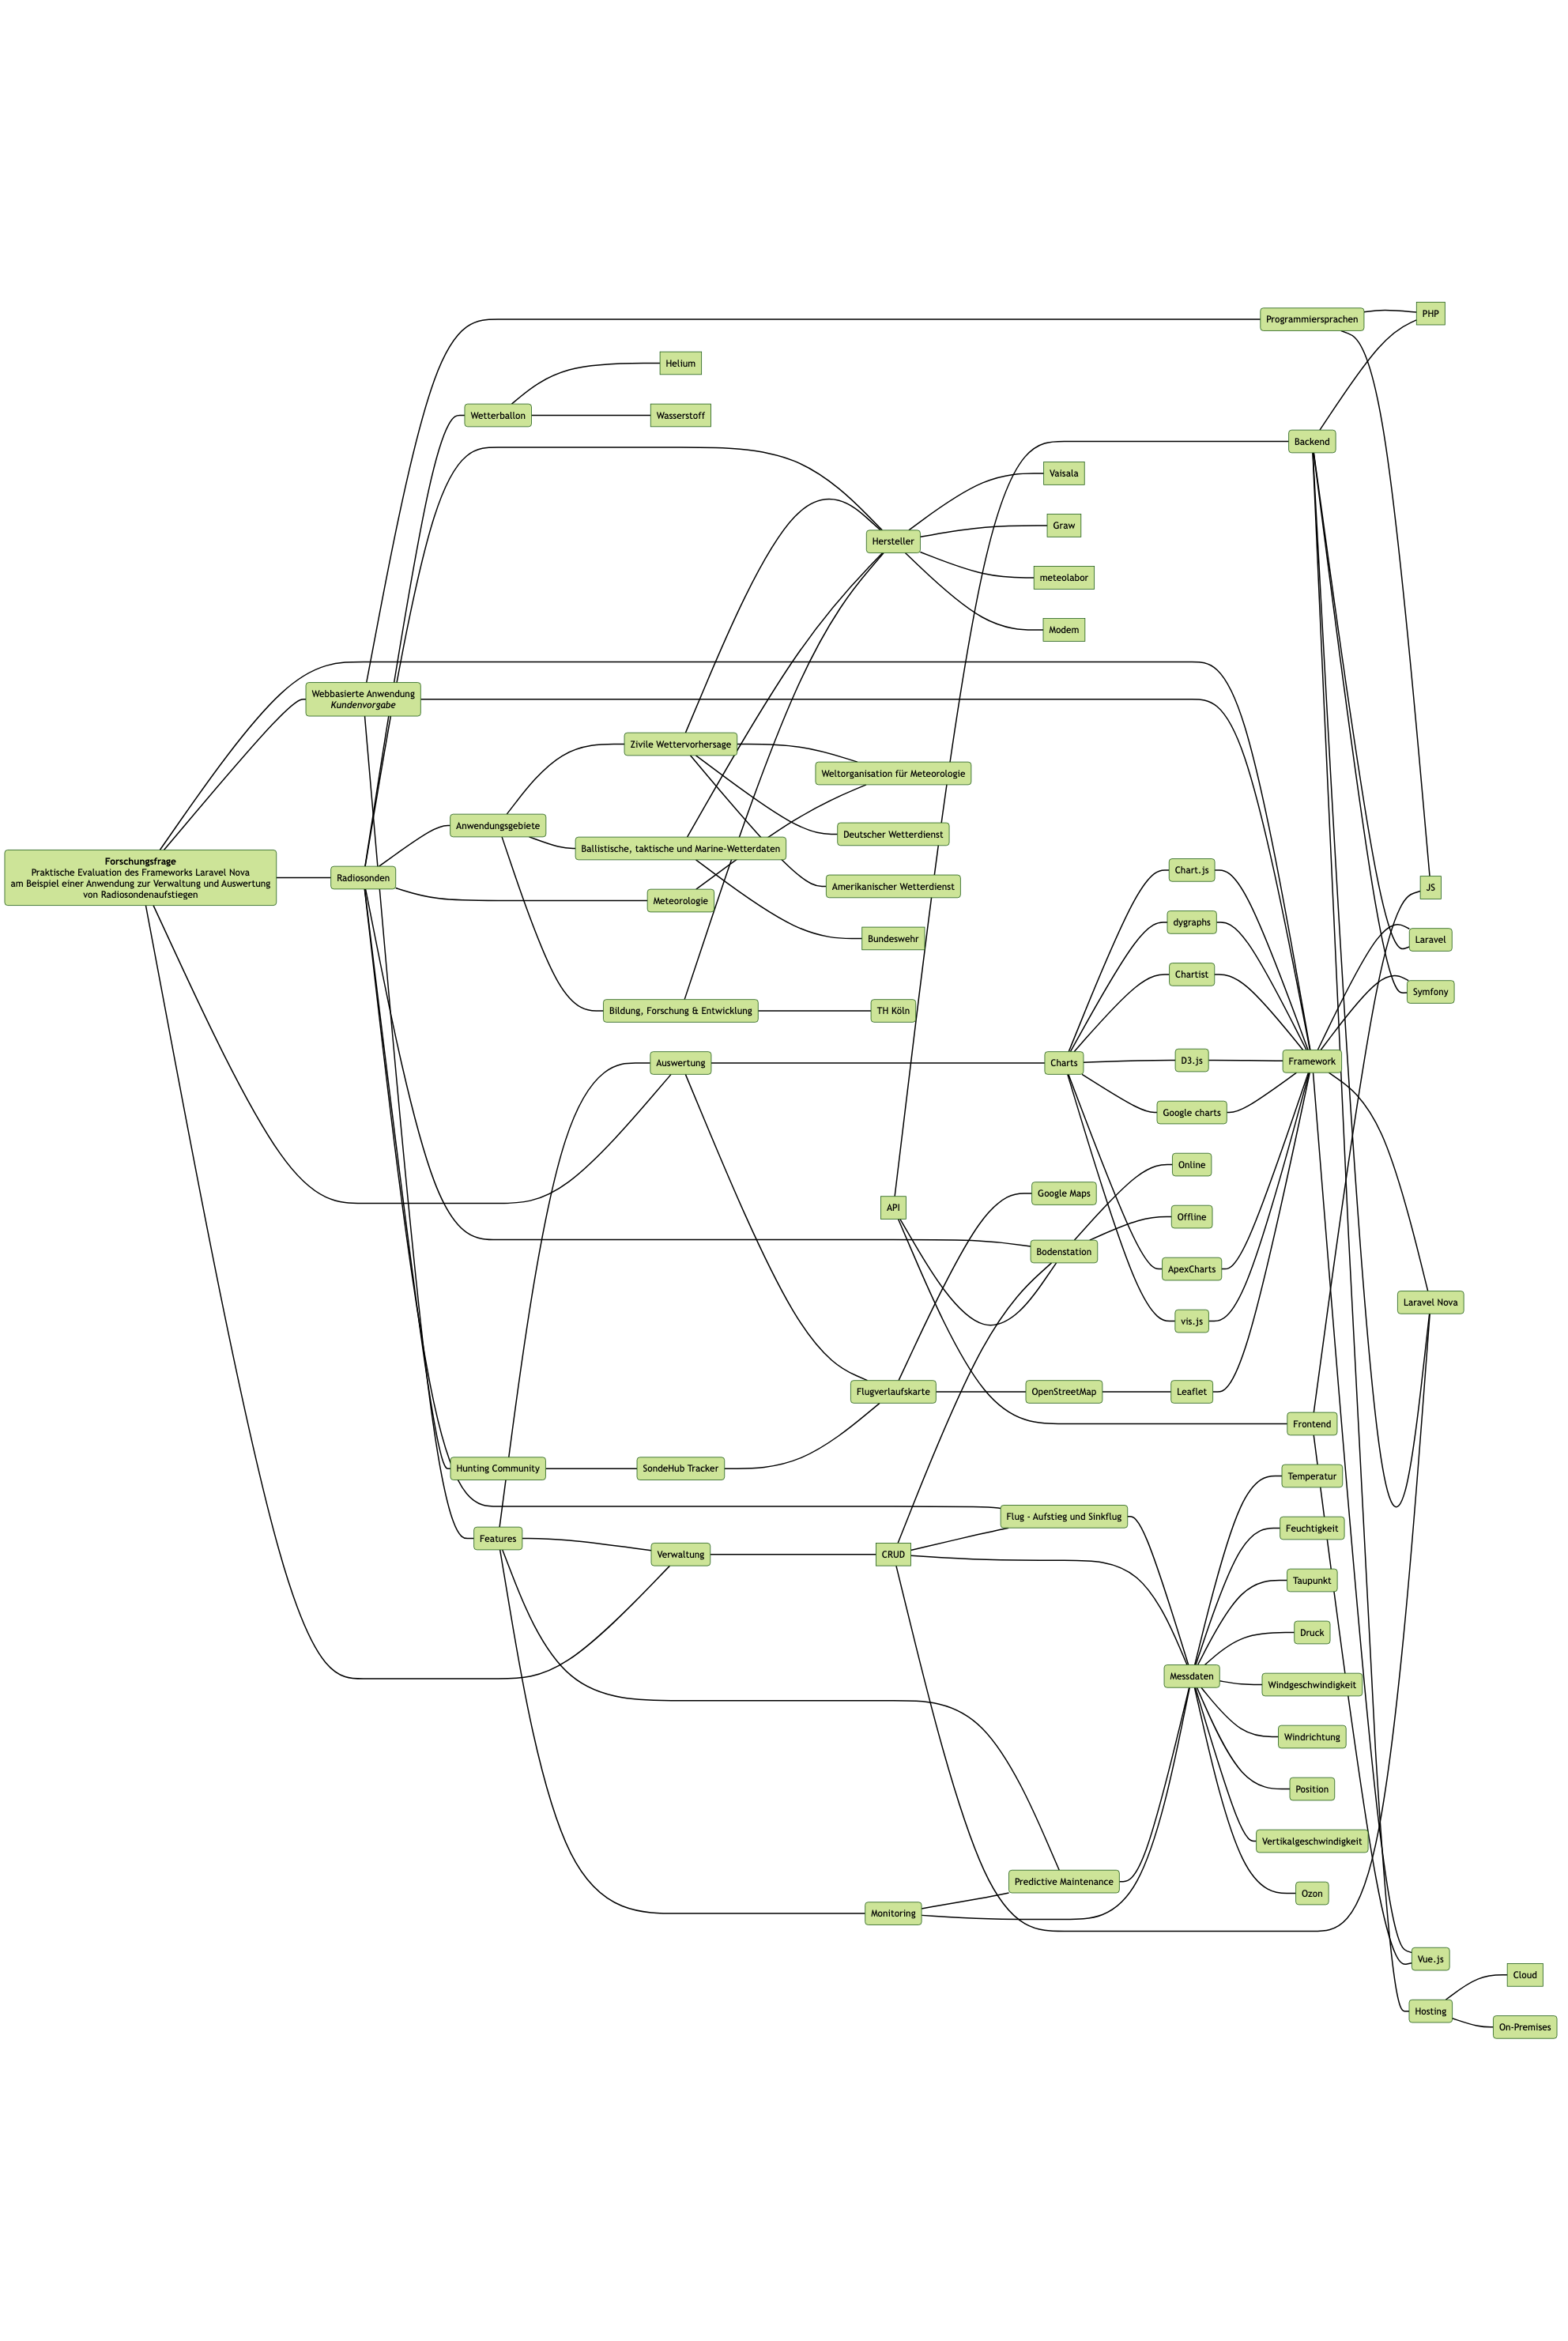
\includegraphics[scale=0.23]{images/themenfeldanalyse}
\end{figure}

    \newpage


\section{Ergebnisse}

Lorem ipsum.\cite{laravel-nova-docs}

    \newpage


\section{Einordnung}

\subsection{Beantwortung der Forschungsfrage}

    \newpage


\section{Fazit}


    \appendix

% Quellenverzeichnis
\newpage


\section{Quellenverzeichnis}
\bibliographystyle{plain}
\printbibliography

% Abbildungsverzeichnis
\newpage
\renewcommand{\listfigurename}{Abbildungsverzeichnis}
\listoffigures

% Tabellenverzeichnis
\renewcommand{\listfigurename}{Tabellenverzeichnis}
\listoftables

% Anhang
\newpage


\section{Anhang}

\subsection{Eigenständigkeitserklärung}
%\frame{\includegraphics[scale=0.183]{assets/eigenstaendigkeitserklaerung}}

\subsection{Leistungspaket}\label{subsec:leistungspaket}
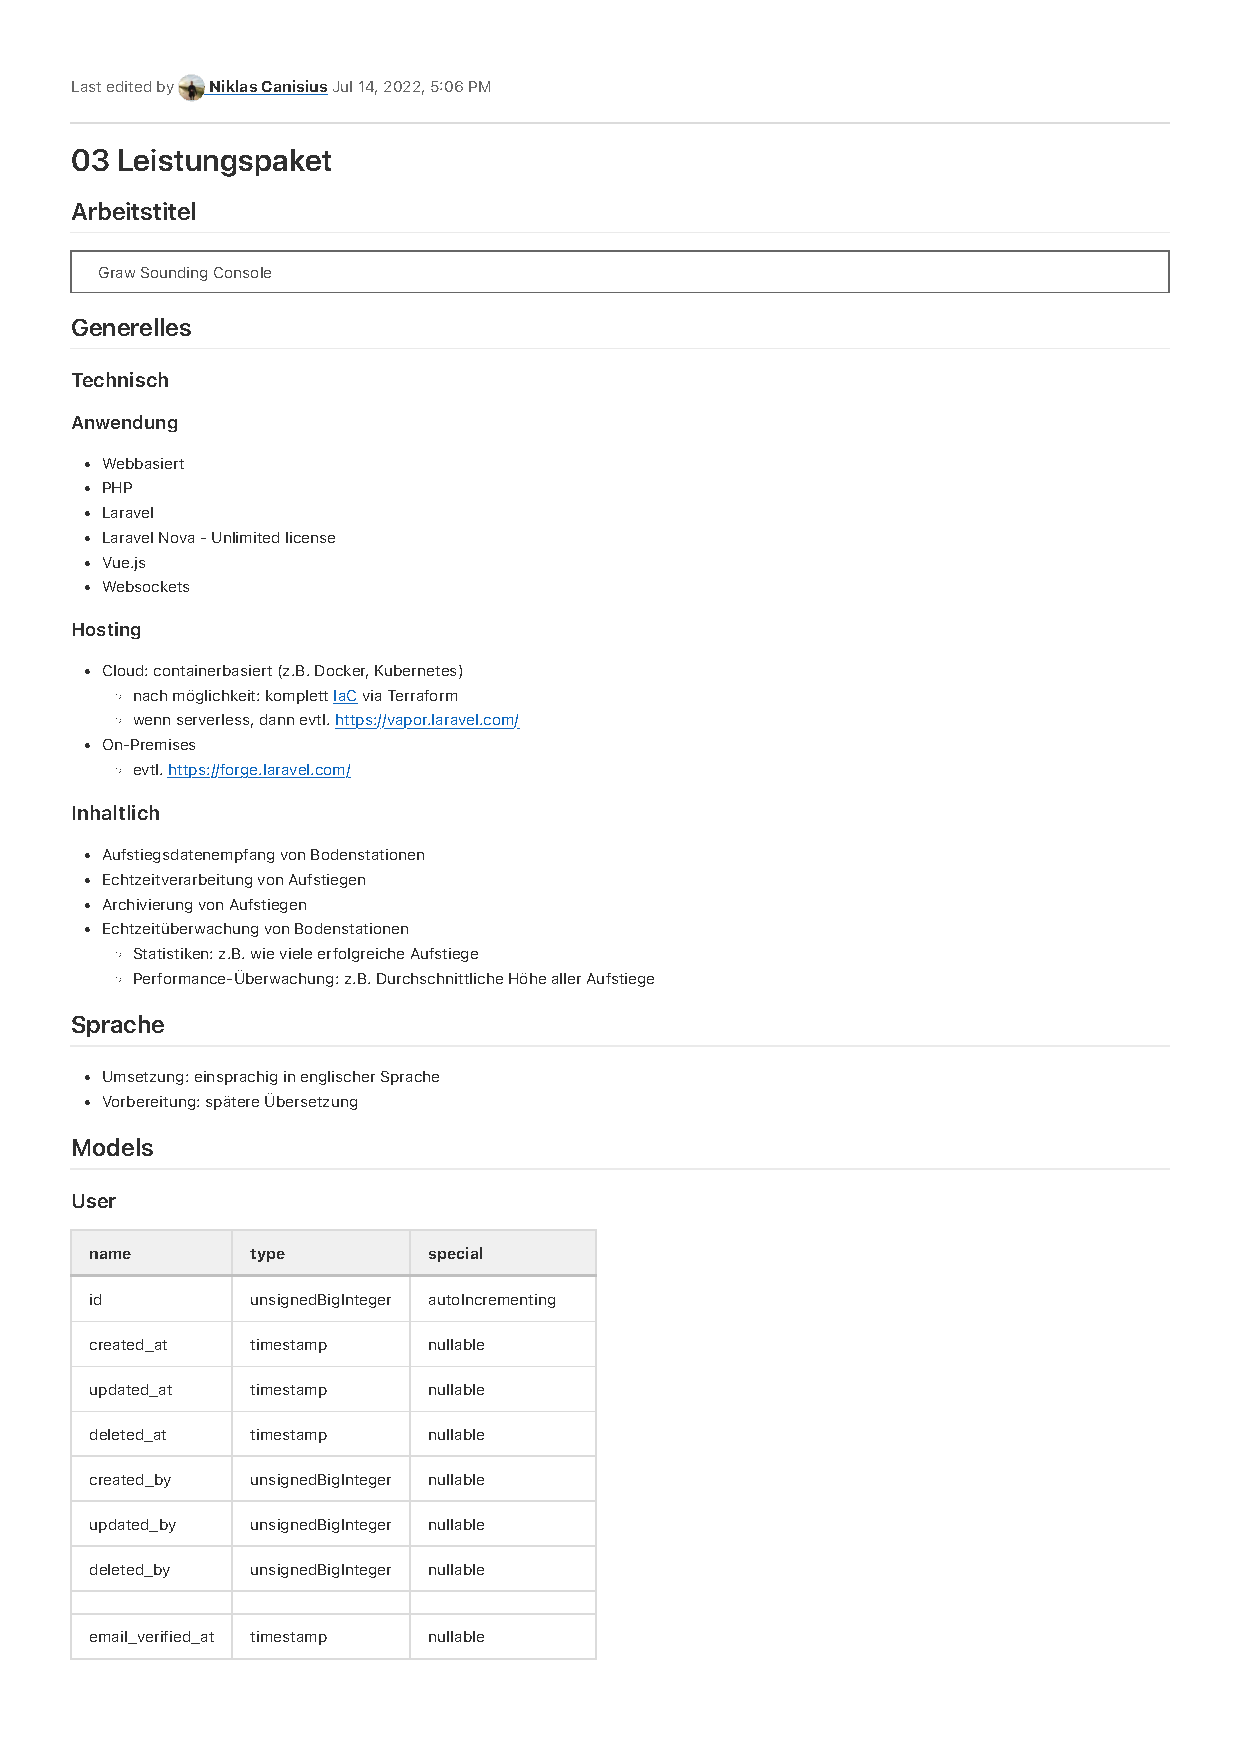
\includepdf[pages=-]{assets/Leistungspaket.pdf}

\subsection{Angebot}\label{subsec:angebot}
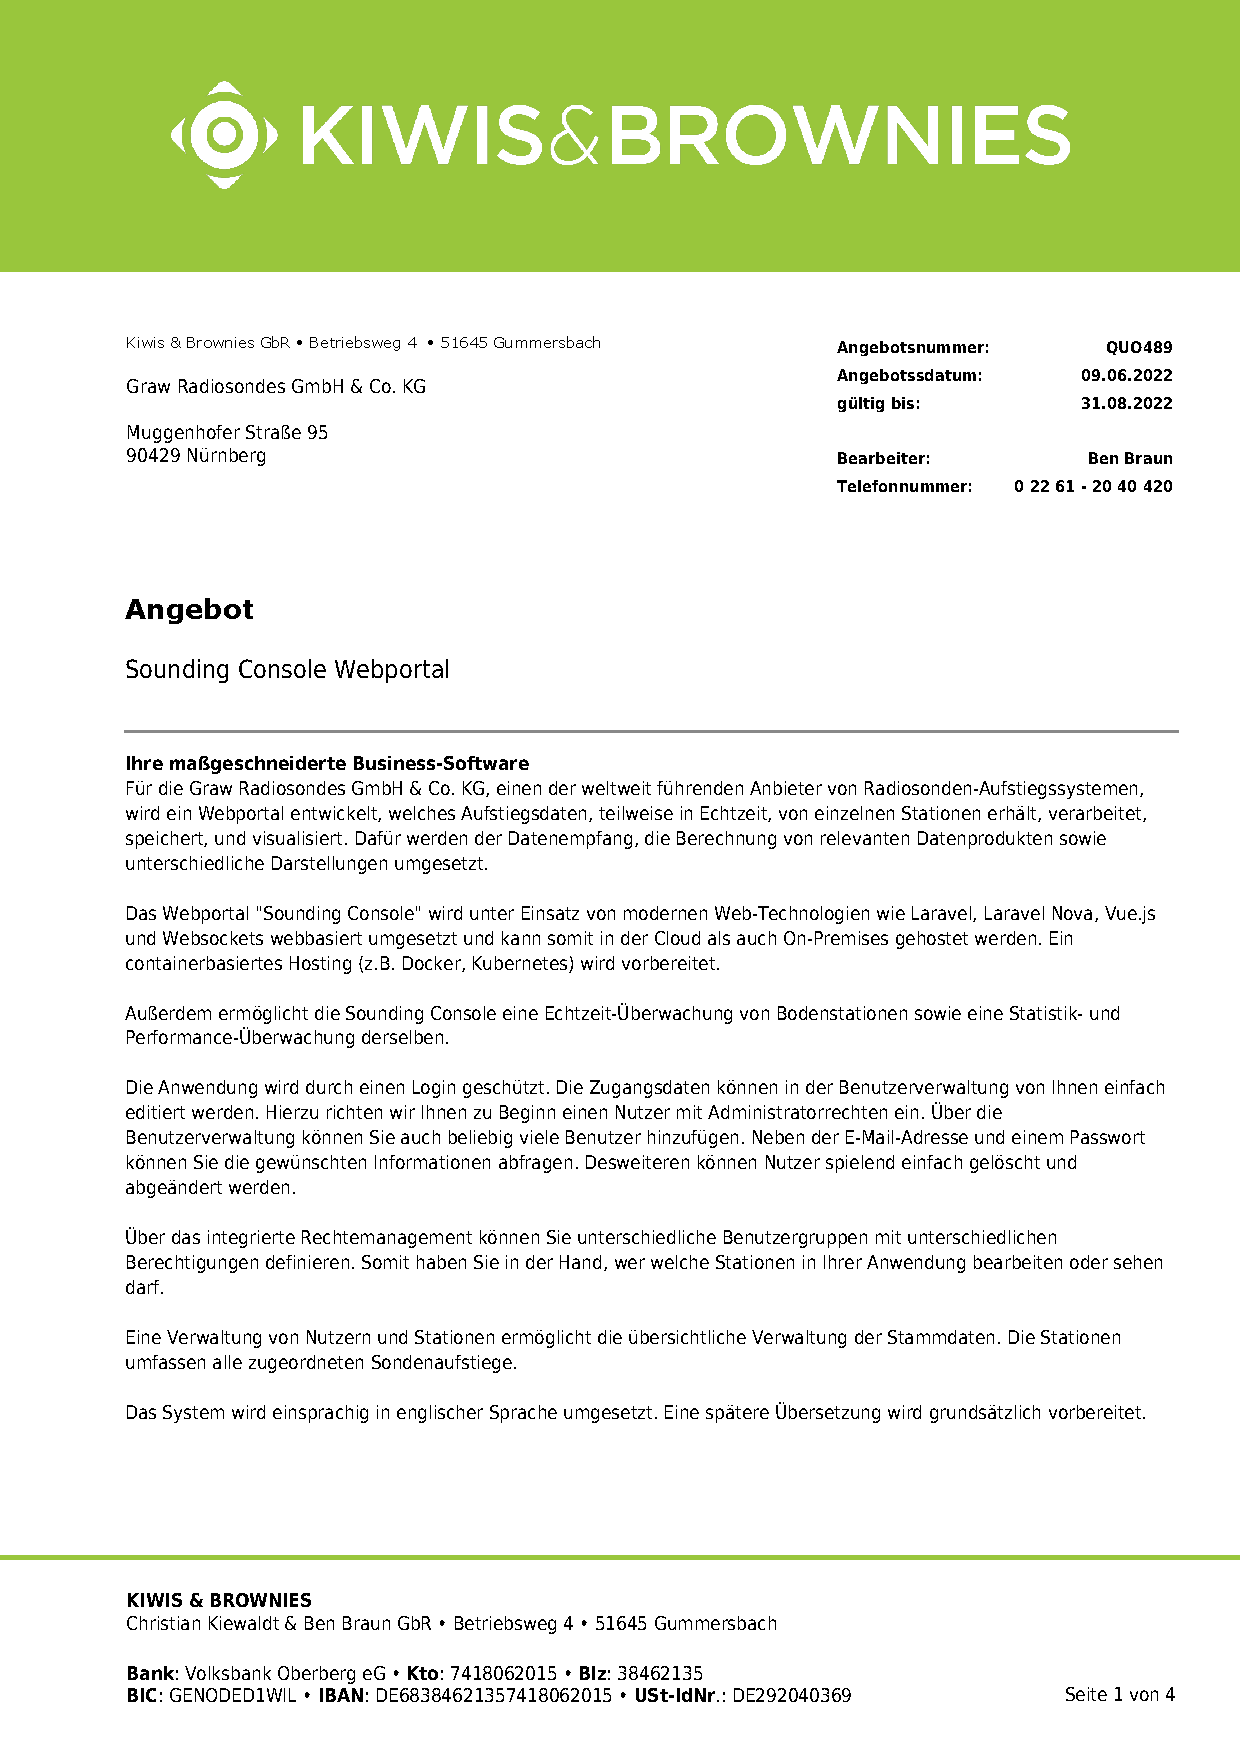
\includepdf[pages=-]{assets/Angebot.pdf}

\subsection{Lastenheft}\label{subsec:lastenheft}
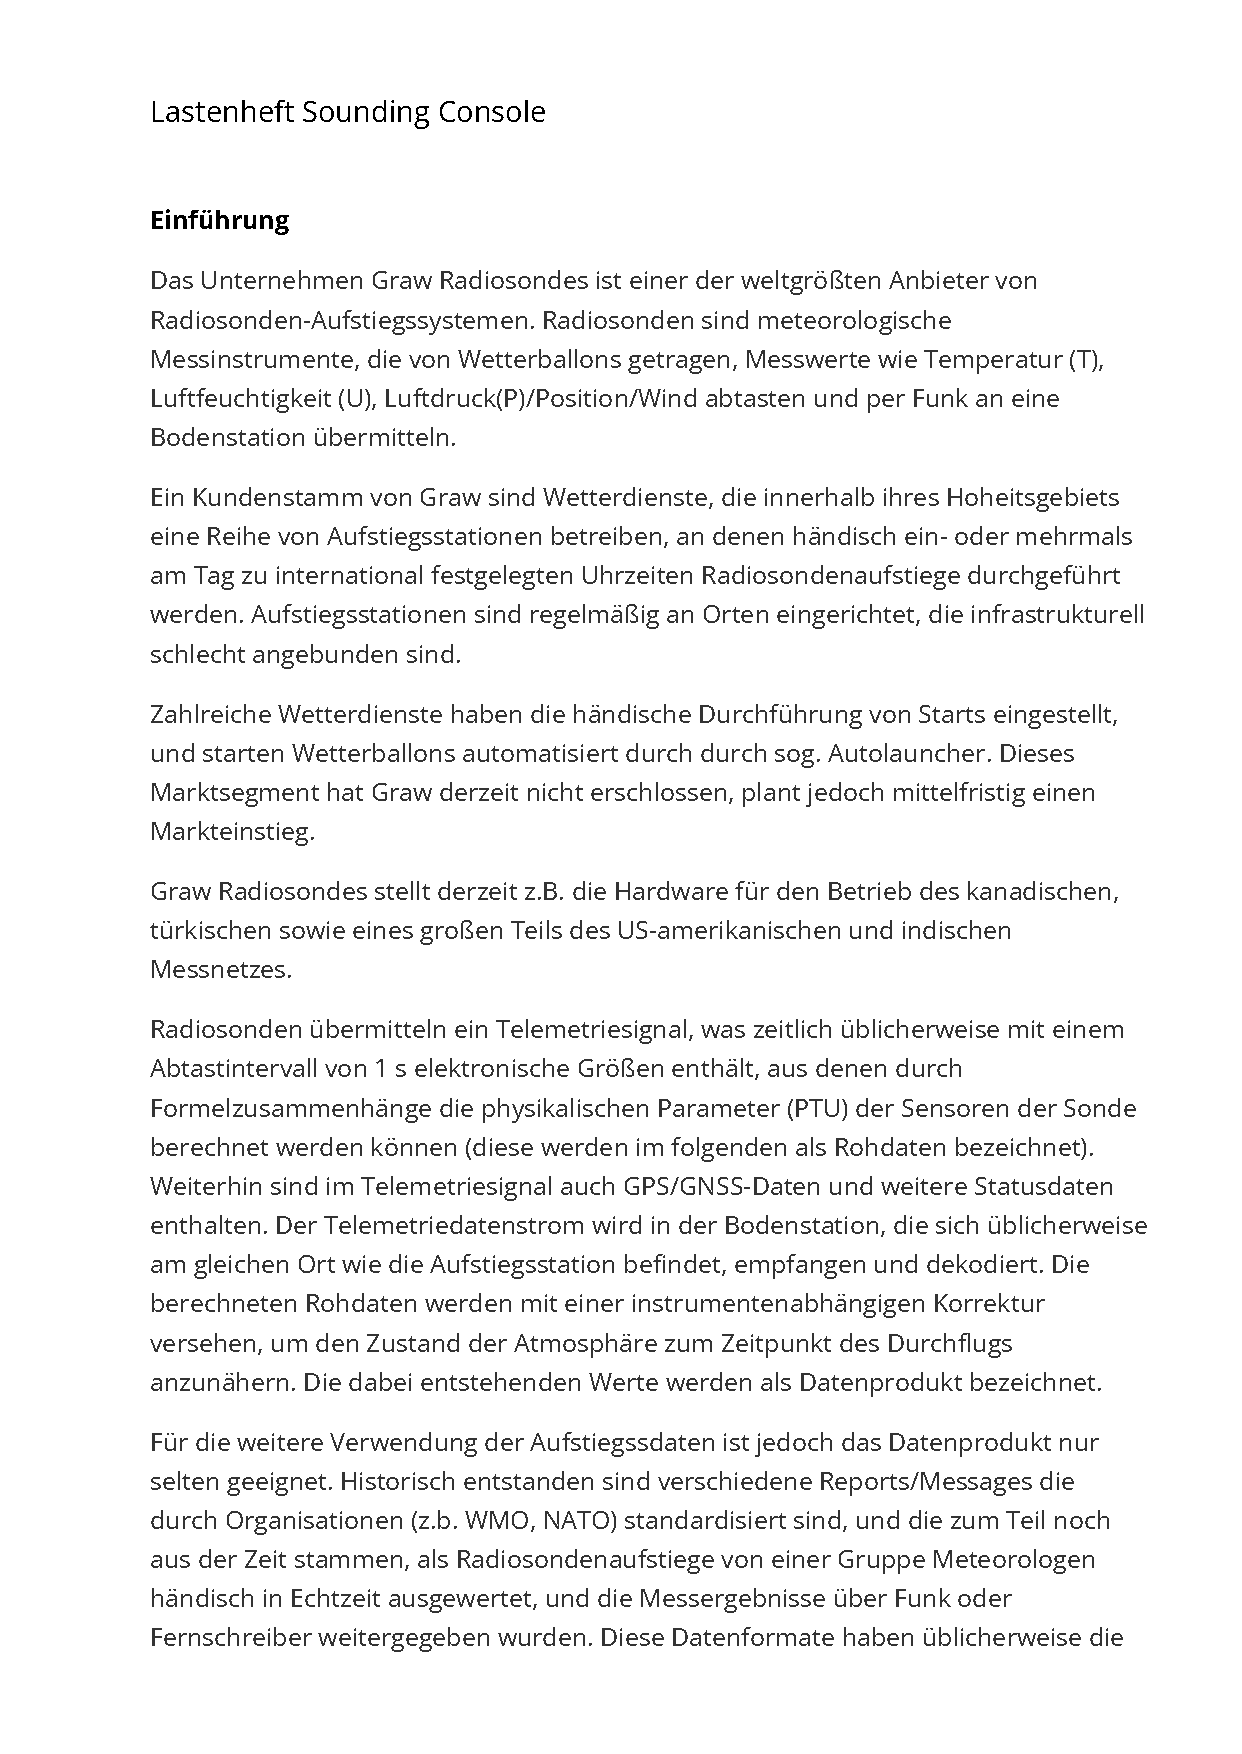
\includepdf[pages=-]{assets/Lastenheft.pdf}

\end{document}
